\chapter{Analyse dans le cadre de théorie de l'information}

Dans cette section, je vais introduire les fondements théoriques de l'approche de la théorie de l'information que j'ai utilisé. Plus particulèrement, la représentation symbolique et les indicateurs : l'entropie et le taux d'entropie d'une séquence symbolique.

\section{Représentation symbolique d'un système dynamique}

Je vais présenter le concept de représentation symbolique d'un système dynamique, i.e., comment extraire des séquences de symboles, qui rendent compte de la complexité du système dynamique d'intérêt, à partir de séries temporelles. Cela dans le but de calculer ensuite l'entropie associée à ce système.

\subsection{Théorie}

La méthodologie sur laquelle repose la démarche scientifique que nous avons choisi d'appliquer pendant mon stage est centrée autour du concept de représentation symbolique. En effet, on souhaite calculer l'entropie relative à différentes conditions expérimentales, i.e., un target word, un mot individuel, issu d'une phrase simple ou bien d'une phrase complexe, pour pouvoir ensuite les comparer entre elles. N'ayant pas accès de manière déterministe à la dynamique cérébrale mais ayant comme mesures de celle-ci les séries temporelles du signal MEG, il n'est pas possible de calculer directement l'entropie. En se basant sur la théorie des systèmes dynamiques \cite{3}, on va donc passer par un système dynamique discret isomorphe au système dynamique d'étude, c'est ce que l'on appelle la représentation symbolique. 

On définit dans un premier temps l'espace des phases (ou espace des états) \cite{18} qui constitue l'espace mathématique dans lequel tous les états possibles d'un système dynamique sont représentés ; chaque état possible correspond à un point unique dans l'espace des phases comme illustré en Figure \ref{fig4.1}. Cet espace permet de nous affranchir du temps en représentant les capteurs les uns en fonction des autres dans un hyperespace, où chacun d'eux représente un degré de liberté du système dynamique étudié, en l'occurence ici, la dynamique cérébrale.

La représentation symbolique peut être vue comme le fait de transformer les trajectoires dans l'espace des phases d'un système dynamique (séries temporelles) en une séquence d'états discrets représentés par un ensemble fini de symboles qui constitue les étiquettes des éléments de la partition. L'ensemble des symboles d'une séquence symbolique est appelé alphabet et correspond à la partition utilisée. Celui-ci est lié à la séquence symbolique et nous donne la trace de la représentation symbolique en question, i.e., la partition qui a été utilisée pour créer des représentations symboliques à partir des séries temporelles du système dynamique étudié.

\begin{figure}[!ht]
    \centering
    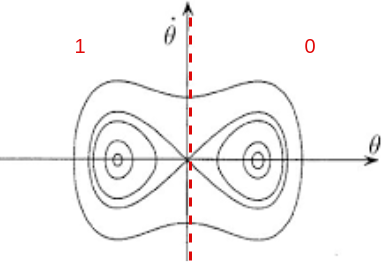
\includegraphics[width=8cm]{representation_symbolique.png}
    \caption{Illustration de la représentation symbolique dans l'espace des phases. Ici représenté en seulement 2 dimenions avec une partition binaire, les points des trajectoires à gauche de la ligne en pointillé rouge sont associés au symbole 1 tandis que ceux à droite sont associés au symbole 0.}
    \label{fig4.1}
\end{figure}

La dynamique symbolique revient donc à échanger des séries temporelles à valeurs continues d'un système dynamique contre des séquences symboliques avec un alphabet fini d'un système dynamique discret, qui sont les représentations symboliques. Les symboles de ces représentations sont les états discrets de la dynamique symbolique. Une séquence symbolique peut donc être vue comme un processus stochastique où la collection de variables aléatoires prend comme valeurs des symboles codés à partir d'un alphabet. En effet, une partition divise l'espace des phases en un nombre fini de régions. Chaque région se voit attribuer un symbole. Toute orbite de longueur infinie peut alors être convertie en une séquence symbolique en enregistrant la région de l'espace des phases que la trajectoire visite à chaque instant. Une représentation symbolique est donc une séquence de symboles qui rendent comptent des états discrets d'un système dynamique au cours du temps par rapport à une partition que l'on souhaite être génératrice dans l'espace des phases (espace des états).

L'entropie d'une séquence symbolique est une mesure qui nous donne énormément de renseignement. Dans le cadre de la théorie de l'information, l'entropie de Shannon nous renseigne sur la production d'information d'une source et l'imprévisibilité de celle-ci. Dans le cadre des systèmes dynamiques, l'entropie de Kolmogorov-Sinai $h_{\mu}(f) = sup h_{\mu}(f,\alpha)$ \cite{3} représente la quantité d'informations nécessaire pour reconstruire une trajectoire dans l'espace des phases à partir d'une condition initiale. Cela nous donne en fait la complexité de la dynamique intrinsèque du système observé et dans quelle mesure celui-ci est chaotique, i.e., désordonné. 

\vspace{2ex}
Le lecteur ou la lectrice trouvera les détails et les définitions mathématiques des concetps que l'on vient d'expliciter en annexe.

\subsection{Pratique}

La première manière de représenter symboliquement la trajectoire associée à notre système dynamique est d'extraire une séquence symbolique pour chaque série temporelle des canaux. Son principe est assez simple et on traite les canaux un par un. En effet, pour chaque canal, on mesure l'amplitude crête à crête du signal pour savoir dans quel intervalle le signal prend ses valeurs. On détermine alors l'histogramme des valeurs du canal en question que l'on va diviser par équipartition. En effet, à partir du nombre de symboles que l'on décide de fixer, i.e. la taille de l'alphabet, on découpe uniformément l'intervalle des valeurs en autant d'intervalles que l'on souhaite de symboles. On effectue ensuite l'attribution des symboles, i.e., les entiers qui sont étiquettes de chaque intervalles, aux points de la série temporel grâce à la fonction digitize du module numpy. 

\begin{figure}[!ht]
    \centering
    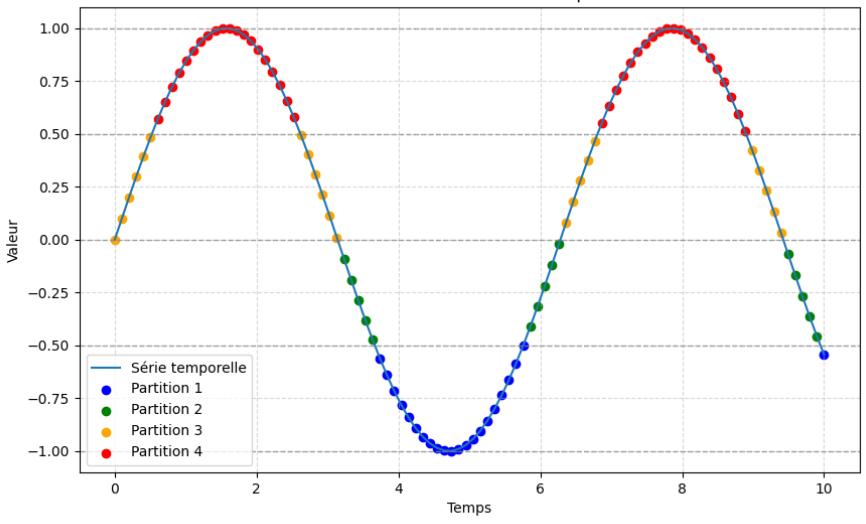
\includegraphics[width=13cm]{partition_serie_temporelle.png}
    \caption{Illustration d'une équipartition par histogramme des valeurs d'une série temporelle. Exemple d'une partition à 4 symboles d'une sinusoïde. On peut identifier les différents intervalles qui correspondent chacuns à un symbole de la partition}
    \label{fig4.2}
\end{figure}

En y associant un alphabet par défaut de la même taille que le nombre de symboles, on a alors une représentation symbolique de chaque canal et il suffit alors de créer les objets séquences symboliques correspondants grâce à la classe sequence du module scikits-symbolic que l'on présentera dans le chapitre suivant.

\vspace{2ex}
La deuxième façon d'effectuer une représentation symbolique de notre système dynamique que nous avons utilisé est une représentation symbolique dans l'espace des phases des capteurs. 
Pour se faire, on effectue une décomposition en valeurs singulières (SVD) \cite{20} de la matrice de nos données (capteurs $\times$ temps), plus précisement, comme la convention est d'avoir une matrice des données (temps $\times$ valeurs), on fait une décomposition en valeurs singulières de la transposée de notre matrice de données.

\vspace{2ex}
Soit $M$ la transposée de la matrice des données $m \times n$, la décomposition en valeurs singulières est définie par 

\begin{equation}
	M = USV^T
\end{equation}

\begin{enumerate}
	\item $U \in \mathcal{R}^{m \times n}$ contient un ensemble de vecteurs orhonormés de $\mathcal{R}^{m}$, dits "de sortie"
	\item $S$ est une matrice diagonale de $\mathcal{R}^{n \times n}$ qui contient les valeurs propres de $M^TM$
	\item $V^T \in \mathcal{R}^{n \times n}$ contient un ensemble de vecteurs orthonormés de $\mathcal{R}^{n}$, dits "d'entrée". Ce sont les vecteurs propres associés aux valeurs propres de $M^TM$ contenus dans $S$
\end{enumerate}

La SVD est une méthode qui permet notamment de faire une réduction de dimension de nos données tout en conservant un maximum d'informations sur la variance de celles-ci. 

\vspace{2ex}
On projette ensuite nos données dans un sous-espace formé par les vecteurs propres ayant les valeurs propres les plus grandes. Le choix du nombre de valeurs propres que nous gardons est fait en fonction du critère de sélection de Schwarz \cite{19} qui revient à regarder le décrochage au niveau de la pente lorsque l'on représente les valeurs propres par ordre décroissant comme on peut l'observer en Figure \ref{fig4.3}. 

\begin{figure}[!ht]
    \centering
    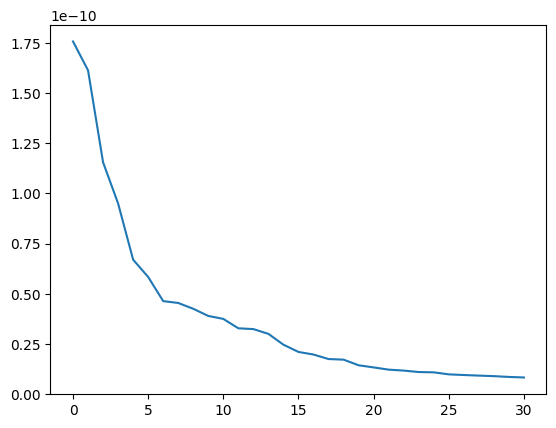
\includegraphics[width=9cm]{30vp.png}
    \caption{Graphe des 30 premières valeurs propres issues de la SVD de la matrice des données pour un sujet de la tâche visuelle}
    \label{fig4.3}
\end{figure}

Dans notre cas, cela revient à prendre les 10 premières valeurs propres. Les vecteurs propres que nous gardons correspondent aux directions selon lesquelles on retrouve le plus d'informations quand à la variabilité des valeurs des champs magnétiques au cours du temps mesurés par les capteurs. Ce sont les vecteurs propres associés aux valeurs propres qui permettent d'expliquer le plus, quantitativement parlant, la variance de nos données. Dans cet espace de moindre dimension, chaque dimension, i.e., chaque valeur singulière, correspond à des combinaisons linéaires des différents capteurs. 

\vspace{2ex}
On ne garde donc qu'une partie $d$ des vecteurs propres contenus dans $V$ de sorte à avoir une matrice $U' \in {R}^{n \times d}$. De la même manière, on crée $S' \in {R}^{d \times n}$ en tronquant $S$ et $V' \in {R}^{n \times d}$. On obtient alors notre matrice des données réduite par $M' = U'S'V'^T$.


\vspace{2ex}
On représente ces nouveaux canaux les uns en fonction des autres, pour former un espace des phases des valeurs singulières des capteurs. C'est dans ce nouvel hyperespace que l'on va déterminer l'histogramme des valeurs selon toutes les dimensions afin de déterminer la partition associée et découper cet hyperespace en autant d'intervalles que l'on souhaite avoir de symboles pour nos représentations symboliques. J'ai illustré cet méthode avec les données d'un sujet de la tâche visuelle en Figure \ref{fig4.4}. 

\begin{figure}[!ht]
    \centering
    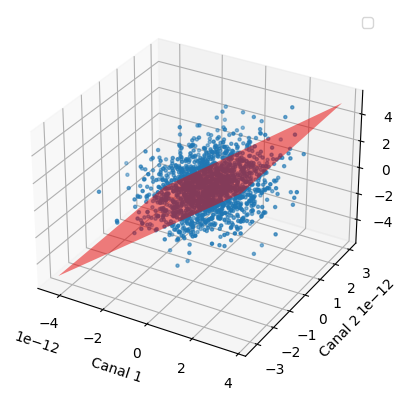
\includegraphics[width=9cm]{representation_espace_des_phases.png}
    \caption{Espace des phases de 3 valeurs singulières avec une partition binaire}
    \label{fig4.4}
\end{figure}

On récupère alors une partition selon chaque axe qui nous permet de créer nos séquences symboliques. 

\vspace{2ex}
Dans le cas où l'on fait une représentation symbolique dans l'espace des phases des données projetées sur une partie des vecteurs propres, i.e., l'espace des phases des valeurs singulières, deux choix s'offre à nous. On peut directement quantifier la dynamique de chaque séquence symbolique ou bien de créer une nouvelle séquence symbolique globale à partir des séquences symboliques obtenues. On obtient alors une séquence symbolique qui représente la dynamique globale du cerveau plutôt que par valeurs singulières, quand bien même quantifier la dynamique de chaque séquence permet d'obtenir un vecteur de taux d'entropie qui quantifie la dynamique cérébrale globale. La création d'une unique séquence symbolique résultante a du sens avec la méthode de représentation symbolique utilisée car les séquences symboliques sont représentées à partir des valeurs singulières des données, i.e., des combinaisons linéaires des capteurs. Pour se faire, on utilise la méthode recode de la classe séquence que l'on détaillera dans le chapitre suivant. Cette fonction permet de créer une séquence symbolique avec un nouvel alphabet à partir de plusieurs séquences symboliques et le fait que leur alphabet soit tous différents.
 
\vspace{2ex}
Que ce soit avec la première méthode ou la seconde, on peut ensuite quantifier la dynamique de chaque séquence symbolique et ainsi comparer la dynamique associée à différentes conditions expérimentales. C'est ce que l'on va approfondir par la suite grâce à la métrique qu'est l'entropie.

\section{Entropie}

Les éléments de la théorie de l'information présentés ci-dessous sont des résultats issus de \cite{2}. On présentera donc seulement les définitions utiles pour notre étude.
Le concept d'entropie a été définie pour la première fois par Shannon en 1948 \cite{21}. Cette quantité est une mesure de l'incertitude d'une variable aléatoire.
Soit $X$ une variable aléatoire discrète ayant $\mathcal{X}$ comme alphabet (ensemble des valeurs ou symboles que peut prendre la variable aléatoire $X$) et $p(x)=Pr\left\{X=x\right\}, x \in \mathcal{X}$ comme fonction de masse de probabilité. 
L'entropie $H(X)$ d'une variable aléatoire discrète $X$ est définie par

\begin{equation}
    H(X) = - \sum_{x \in \mathcal{X}} p(x)logp(x)
\end{equation}

Lorsqu'on s'intéresse à une seule variable aléatoire $X$, on peut aussi noter l'entropie $H(p)$ où $p$ désigne la fonction de masse de probabilité de la variable $X$.
Le $log$ est en base 2, l'unité de l'entropie est donc le bit. Il est d'usage d'également utiliser le logarithme népérien en base e pour d'autres domaines que la compression et la transmission de données. En fonction de la base du logarithme choisie, si par exemple celle-ci est $b$, on notera l'entropie associée $H_b(X)$. 

Voici quelques propriétés importantes de l'entropie :
\begin{enumerate}
    \item $H(X)\geq0$
    \item $H(p)$ est une fonction concave de p.
    \item $H_b(X)=(log_{b}a)H_{a}(X)$
\end{enumerate}

Illustrons la notion d'entropie et ses proprétés de base avec un exemple simple, celui d'un tirage aléatoire binaire \cite{8}. Comme on peut l'observer sur la Figure \ref{fig4.5}, on a $H(p)=0$ lorsque $p=0$ ou $p=1$ et $H(p)=1$ lorsque $p=1/2$. Cela revient à dire que l'entropie est nulle lorsque la variable n'est plus aléatoire (i.e. non incertaine) et que l'entropie atteint sa valeur maximale lorsque l'incertitude est maximale.

\begin{figure}[!ht]
    \centering
    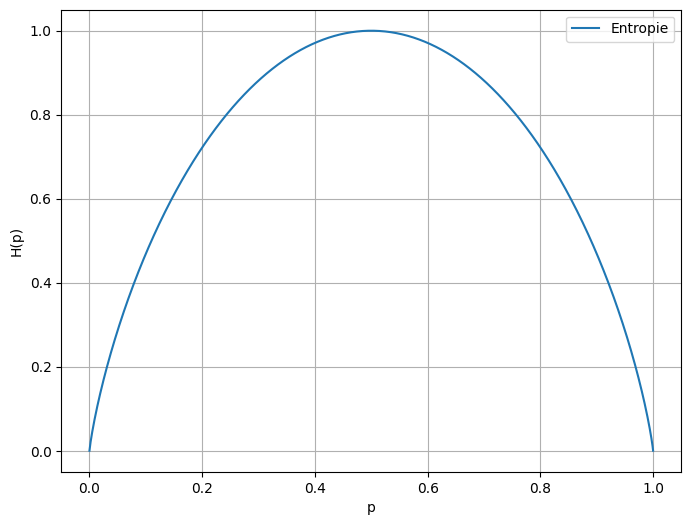
\includegraphics[width=9cm]{exemple_entropie.png}
    \caption{Entropie $H(p)$ en fonction de la probabilité $p$ d'un événement binaire}
    \label{fig4.5}
\end{figure}

En considérant une paire de variables aléatoires discrètes $(X,Y)$ de distribution joint $p(x,y)$ comme une seule variable aléatoire vectorielle, on obtient aisèment la définition de l'entropie jointe $H(X,Y)$ par

\begin{equation}
    H(X,Y) = \sum_{x \in \mathcal{X}}\sum_{y \in \mathcal{Y}}p(x, y)logp(x,y)
\end{equation}

On peut également définir l'entropie conditionnelle d'une variable aléatoire sachant une autre variable aléatoire comme la moyenne par rapport à la variable aléatoire de conditionnement des entropies des distributions conditionnelles.
Si $(X,Y) \sim p(x,y)$, alors l'entropie conditionnelle $H(Y|X)$ est donnée par 

\begin{equation}
    H(Y|X) = \sum_{x \in \mathcal{X}}p(x)H(Y|X=x) = -\sum_{x \in \mathcal{X}}p(x)\sum_{y \in \mathcal{Y}}p(y|x)logp(y|x)
\end{equation}

Ainsi, on a

\begin{equation}
    H(Y|X) = -\sum_{x \in \mathcal{X}}\sum_{y \in \mathcal{Y}}p(x,y)logp(y|x)
\end{equation}

L'entropie jointe et l'entropie conditionnelle d'une paire de variables aléatoires sont reliées par :

\begin{equation}
    H(X,Y) = H(X) + H(Y|X)
\end{equation}

Ce qui nous permet d'introduire la règle de la chaîne pour l'entropie.
Afin de pouvoir définir le taux d'entropie d'un processus stochastique dans la section suivante, on généralise la règle de la chaîne pour une collection de $n$ variables aléatoires. En effet, l'entropie d'une collection de variables aléatoires est défini par la somme des entropies conditionnelles.

Soit $X_1, X_2, ...,X_n$ une collection de variables aléatoires distribuées selon $p(x_1, x_2, ...,x_n)$. 

\vspace{2ex}
On a alors

\begin{equation}
    H(X_1, X_2, ...,X_n)= \sum_{i=1}^{n}H(X_i|X_{i-1},...,X_1) \label{eq:chaine}
\end{equation}

\vspace{2ex}
Nous allons à présent détailler notre démarche quand au calcul du taux d'entropie d'une séquence symbolique.

\section{Processus stochastique et taux d'entropie}

Les séquences symboliques extraites à partir des segments temporels des données MEG peuvent donc être considérées comme des processus stochastiques.

D'après \cite{2}, un processus stochastique $\textbf{Z}=\{Z_i \}$ est une séquence indexée de variables aléatoires. En général, il peut y avoir une dépendance arbitraire entre les variables aléatoires. Le processus est caractérisé par les fonctions de masse de probabilité conjointes

\begin{equation}
    Pr\{(Z_1, Z_2, ...,Z_n)=(z_1, z_2, ...,z_n)\}=p(z_1, z_2, ...,z_n)
\end{equation},
$(z_1, z_2, ...,z_n) \in \mathcal{Z}^n$ pour $n=1,2,...$

\vspace{2ex}
Une caractéristique importante d'un processus stochastique est la stationnarité. Un processus stochastique est dit \textit{stationnaire} si la distribution conjointe de tout sous-ensemble de la séquence de variables aléatoires est invariante par rapport aux changements de l'indice de temps ; c'est-à-dire,

\begin{equation}
    Pr\{Z_1=z_1,Z_2=z_2,..., Z_n=z_n \} = Pr\left\{Z_{1+l}=z_1,Z_{2+l}=z_2,..., Z_{n+l}=z_n \right\}
\end{equation}

Dans notre cas, on fera l'assomption que les séquences symboliques extraites des données MEG sont des processus stochastiques stationnaires. En effet, la représentation symbolique du signal en entier ne peut pas être considéré comme un processus stochastique mais il est stationnaire par morceaux, i.e. localement stationnaire. En choisissant des segments temporels courts (1.4 sec) centrés sur des événements clairement identifiés (comme par exemple l'apparition sur l'écran d'un target word lors de la tache visuelle), on peut considérer les représentations symboliques extraites de ces segments comme stationnaires.

On a vu dans la partie précédente, que l'on pouvait calculer l'entropie d'une collection de variables aléatoires $H(Z_1, Z_2, ...,Z_n)$ (5.7). On s'intéresse à la limite lorsque n tend vers l'infini de cette métrique que l'on appelle taux d'entropie. Le taux d'entropie permet de mesurer des structures de réccurence et donc la production d'information de la source, c'est l'accélération de l'entropie.
Le taux d'entropie d'un processus stochastique  $\textbf{Z}=\{Z_i \}$ est alors défini d'après \cite{2} par

\begin{equation}
    H(\textbf{Z})=\lim_{n \to \infty}\frac{1}{n}H(Z_1, Z_2, ...,Z_n) \label{eq:taux1}
\end{equation}

Quand la limite existe. 
Ce taux d'entropie correspond à la limite des entropies par symboles des variables aléatoires. 

On peut aussi définir une quantité liée pour le taux d'entropie \cite{2} d'après \eqref{eq:chaine} telle que 

\begin{equation}
    H'(\textbf{Z})=\lim_{n \to \infty} H(Z_n|Z_{n-1},Z_{n-2}...,Z_1) \label{eq:taux2}
\end{equation}

Lorsque la limite existe.
Cette deuxième notion du taux d'entropie correspond à la limite de l'entropie conditionnelle de la dernière variable aléatoire du processus stochastique sachant les états des variables aléatoires précédentes.
Pour un processus stochastique stationnaire, les limites convergent et on a égalité entre les deux taux.

\begin{equation}
    H(\textbf{Z}) = H'(\textbf{Z}) = h \label{eq:convergence1}
\end{equation}

Ce résultat est asymptotique alors que nous disposons d'un jeu de données fini et donc de séquences symboliques finies. Il en va de déterminer le taux d'entropie en utilisant un estimateur, c'est ce que nous allons présenter maintenant. 

\section{Estimateur de Lempel-Ziv}

L'ultime partie de notre algorithme est le calcul du taux d'entropie des séquences symboliques issues des séries temporelles des données MEG. Le taux d'entropie étant asymptotique et les séquences que l'on génère étants finies, on va donc utiliser un estimateur de cette quantité. Nous avons décidé d'utiliser l'estimateur de Lempel-Ziv \cite{1}. En effet, les séquences symboliques extraites à partir des époques des séries temporelles MEG contiennent 1200 symboles et la convergence de la complexité de Lempel-Ziv vers le réel taux d'entropie a été prouvée \cite{1} pour de courtes séquences, i.e., des séquences de moins de 1000 symboles. De plus, c'est un estimateur sans paramètres libres qui constitue une véritable mesure du taux d'entropie. Enfin, l'estimateur de Lempel-Ziv avait déjà été implémenté par Jean-Luc Blanc et Laurent Pezard dans le module scikits-symbolic. C'est pour ces raisons que nous avons choisi d'utiliser cet estimateur du taux d'entropie. Nous allons à présent expliquer son fonctionnement.

\vspace{2mm}
Considérons une source stationnaire qui émet à chaque pas de temps un symbole d'un alphabet de taille finie $k$. Son entropie de bloc d'ordre $n$ est définie comme l'entropie de Shannon de la distribution de probabilité $p_n(w)$ des mots de longueur $n$ (i.e. des mots de n symboles),

\begin{equation}
    H_n = - \sum_{w}p_n(w)lnp_n(w)
\end{equation}

\begin{enumerate}
	\item $w$ mot de longueur n
	\item $p_n(w)$ distribution de probabilité
\end{enumerate}

Cette somme est calculée sur tous les mots de longueur $n$ possibles $w$, et dépend donc de la dynamique de la source sur les $n$ intervalles de temps.
En conséquence, $h_n = H_{n+1} - H_n$ converge vers une limite $h$ lorsque la longueur des mots tend vers $\infty$, ce qui correspond au taux d'entropie de la source.

\begin{equation}
    h = \lim_{n \to \infty}\frac{H_n}{n} = \lim_{n \to \infty}H_{n+1} - H_n \label{eq:convergence2}
\end{equation}

Ces deux définitions du taux d'entropie correspondent dans l'ordre aux définitions établis en \eqref{eq:taux1} et en \eqref{eq:taux2} d'après \cite{2}. Les équations \eqref{eq:convergence1} et \eqref{eq:convergence2} sont donc équivalentes.

\vspace{2ex}
En pratique, le taux d'entropie $h$ doit le plus souvent être estimé à partir d'une seule séquence observée $[s] = (s_i)_{1 \geq i \geq N}$ de longueur $N$. 
Nous désignerons dorénavant $\hat{X}$ comme l'estimateur d'une quantité $X$, sans mentionner explicitement qu'il dépend de la séquence $[s]$ et de sa longueur $N$. Regarder la limite du taux d'entropie lorsque $n$ tend vers l'infini revient à observer la limite de cette même quantité lorsque $N$ tend vers l'infini.

\vspace{2ex}
Le point de vue adopté pour calculer la complexité de Lempel-Ziv est a priori très différent de celui associé au taux d'entropie de Shannon $h$. En effet, la définition du taux d'entropie de Shannon $h$ implique une caractéristique globale de la dynamique, à savoir sa mesure invariante. Elle peut être calculée à partir de la connaissance d'une seule trajectoire tant que la mesure est ergodique et permet de reconstruire la distribution de probabilité de la source à partir de l'observation d'une seule séquence typique. Mais elle n'est pas, en soi, significative en tant que caractéristique d'une séquence unique. En revanche, la complexité de Lempel-Ziv fournit une mesure de la compressibilité de la séquence symbolique unique considérée, en d'autres termes, le contenu de l'information par symbole. Dans l'hypothèse où la source est stationnaire et ergodique, les théorèmes de Lempel-Ziv \cite{16} garantissent que la complexité de Lempel-Ziv coïncide avec $h$ jusqu'à un facteur $lnk$ impliquant le nombre $k$ de symboles de l'alphabet (la partition utilisée) comme défini en \eqref{eq:lempelziv}. Cette hypothèse implique en effet que presque toutes les séquences symboliques ont les mêmes caractéristiques de compressibilité ; le calcul peut donc être effectué de manière équivalente avec n'importe quelle séquence typique et son résultat coïncide avec la moyenne.

Selon le schéma de Lempel-Ziv, la séquence de longueur $N$ est découpée en $\mathcal{N}_w$ mots. Deux manière de découper la séquence et donc de construire le dictionnaire de mots ont été proposées. On utilisera la première manière de créer des mots à partir des symboles de la séquence, publié en 1976 \cite{15}, qui considère comme mot le plus court ensemble de symboles qui n'a pas encore été rencontré lors du balayement de la séquence. Par exemple :

\begin{equation}
    1 \cdot 0 \cdot 01 \cdot 11 \cdot 100 \cdot 101 \cdot 00 \cdot 010 \cdot 11... .
\end{equation}

Une fois le dictionnaire de mots construit à partir de la séquence, on calcule 

\begin{equation}
    \hat{L} = \frac{\mathcal{N}_w[1 + log_k\mathcal{N}_w]}{N}
\end{equation}

où

\begin{equation}
    \lim_{n \to \infty} \hat{L} = \frac{h}{lnk} \label{eq:lempelziv}
\end{equation}

\begin{enumerate}
	\item $k$ taille de l'alphabet
	\item $\mathcal{N}_w$ nombre de mots du dictionnaire
	\item $N$ taille de la séquence symbolique
\end{enumerate}

C'est donc de cette manière que nous avons calculé la complexité de Lempel-Ziv $\hat{L}$, qui nous donne une très bonne estimation du taux d'entropie d'une séquence symbolique. L'algorithme de Lempel-Ziv que nous avons utilisé fait partie du module scikits-symbolic sur lequel j'ai apporté une contribution et que je vais présenter dans le prochain chapitre.
